\documentclass[9pt]{beamer}

\usetheme[{titleformat plain}=smallcaps,
           titleformat title=smallcaps,
           titleformat subtitle=regular,
           titleformat section=smallcaps,
           titleformat frame=smallcaps,
           numbering=fraction,
          ]{metropolis}
\usepackage{appendixnumberbeamer}
\geometry{paperwidth=213.3mm,paperheight=120mm}

\usepackage{../_style/common}
\usepackage{../_style/defs}
\usepackage{emoji}

\graphicspath{{pictures/}{../_pictures/}}

\title{Data and Interfaces}
\subtitle{
    \itshape
    successful abstractions as building blocks
}
\date{October, 2022}
\author{Alessandro Candido}
\titlegraphic{
    \vfill\vspace*{250pt}
    
\includegraphics[height=1cm]{../_logos/unimi_logo.png}\hfill
    
\includegraphics[height=1cm]{../_logos/infn_logo.png}\\
}

\begin{document}

\maketitle

\setlist[description]{font=\quad\normalfont\bfseries\scshape\space}
\metroset{block=fill}


\begin{frame}{Who am I?}
    \vspace*{30pt}
    \begin{columns}
        \begin{column}{0.03\textwidth}
        \end{column}
        \begin{column}{0.47\textwidth}
            I am a \textbf{PhD student} in \textbf{HEP theory}, about to
            finish.\newline

            Since my Master I have spent a significant part of my research
            working on \alert{\textbf{software projects}}, with an increasing
            number of collaborators.\newline

            \vspace*{5pt}
            \partitle{References}
            \vspace*{5pt}

            Now, as part of \nnpdf{}, I had to work and organize projects with
            $\order{5\text{-}10}$ developers -- not incredibly many, but already
            \textit{\textbf{challenging}}.\newline

            Moreover, personal projects driven me to explore beyond the
            boundaries of what is useful for physics.
            With less \sout{pressure} needs you can explore more\dots but often
            not as deep.\newline

            \vspace*{5pt}
            \partitle{My Goal}
            \vspace*{5pt}

            I am not here to teach, but just to \textbf{share my experience}.
            This is compliant with the references.
        \end{column}
        \begin{column}{0.5\textwidth}
            \begin{figure}
                \centering
                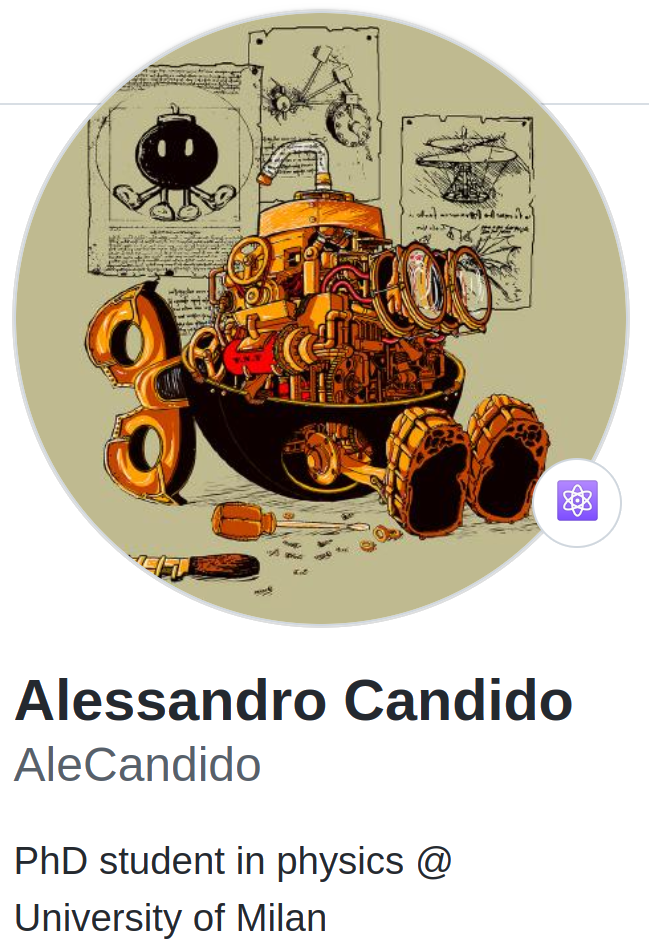
\includegraphics[width=0.5\textwidth]{mygh}
            \end{figure}
        \end{column}
    \end{columns}
\end{frame}

% \begin{frame}{The Role of Trade-offs}
    % \begin{columns}
        % \begin{column}{0.5\textwidth}
            % \vspace*{20pt}
            % \begin{center}
                % \itshape\bfseries 
                % There are no absolute truths.
            % \end{center}
            % \begin{flushright}
                % \itshape
                % -- is this an absolute truth? \emoji{thinking-face}
            % \end{flushright}

            % \vspace*{10pt}
            % In a sense, problems might look similar, even when they are not
            % that much\dots
            % \vspace*{20pt}
            
            % \begin{figure}
                % \centering
                % 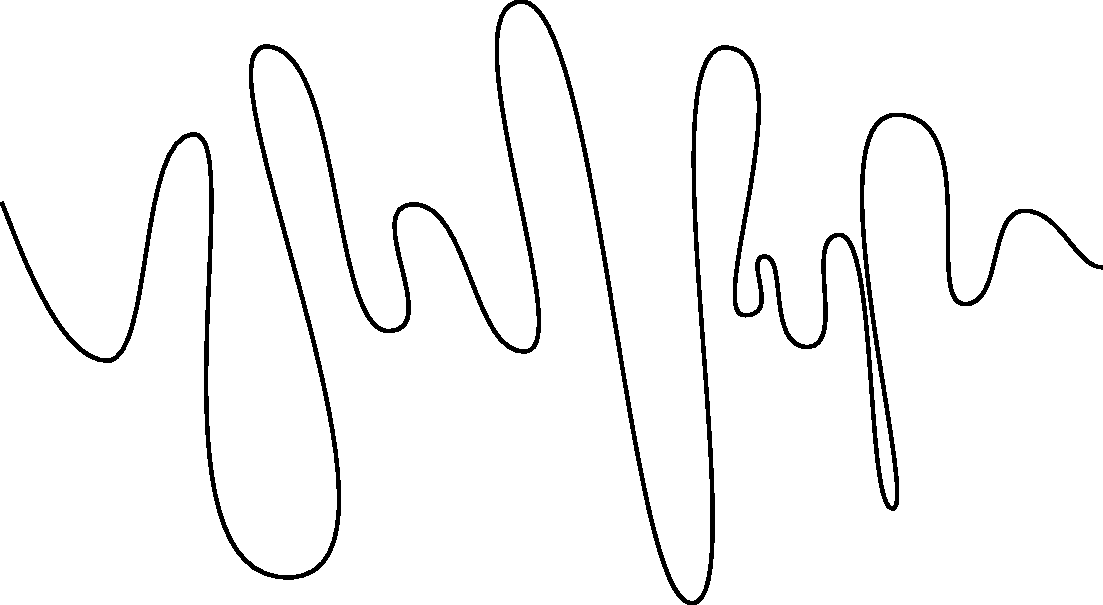
\includegraphics[width=\textwidth]{solution}
                % \caption{
                    % Artistic view of the solution function, over the space of
                    % problems.
                % }
            % \end{figure}
        % \end{column}
        % \begin{column}{0.5\textwidth}
            % So, better to know many possible solutions, and always consider
            % multiple alternatives.

            % \vspace*{10pt}
            % \begin{figure}
                % \centering
                % 
\includegraphics[width=0.6\textwidth]{balancing}
            % \end{figure}
            % \vspace*{10pt}

            % Moreover
            % \href{https://en.wikipedia.org/wiki/All_that_glitters_is_not_gold\#In_popular_culture}{\enquote{All
            % that is gold does not glitter}}, not all good solutions are
            % manifest.
        % \end{column}
    % \end{columns}
% \end{frame}

\begin{frame}{Outline}
    \vspace*{10pt}
    \begin{center}
        \itshape
        The task I have been given is to discuss \textbf{interfaces} and
        \textbf{data management.}
    \end{center}
    \vspace*{10pt}

    \begin{columns}
        \begin{column}{0.5\textwidth}
            \alert{\textbf{Python}} is not the \enquote{best} programming
            language, nor the unique one.
            But Python is definitely a successful one.
            \vspace*{10pt}

            And the success for a language is mostly determined by the
            availability of \textbf{libraries} and
            \textbf{applications}\footnote{
                There are relevant and determinant language features, and for
                Python is its \textbf{expressiveness}, that is fundamental for
                new users and \textit{\textbf{maintainability}}.
            }.\newline

            In the case of Python:
            \begin{description}
                \item[application] scientific computation, and data science\footnote{
                    Part of the success has been due to \textit{web
                    frameworks}, but it is less relevant nowadays.
                }
                \item[libraries] Numpy, Scipy, Pandas, Xarray, \dots
            \end{description}
            \vspace*{30pt}

            Of course ML frameworks now play a big a role, but it is almost a
            consequence\dots
            \vspace*{5pt}
        \end{column}
        \begin{column}{0.5\textwidth}
            So, in a sense, the advantage of Python is that its
            \alert{\textbf{libraries}} can be \alert{\textbf{written not in
            Python}}.

            But in order this to be possible, it is crucial to build a
            successful \textbf{abstraction}.
            \vspace*{20pt}

            \begin{enumerate}
                \item abstractions
                \item interfaces
                \item examples
                \item project management
            \end{enumerate}
            \vspace*{20pt}

            \begin{figure}
                \centering
                
\includegraphics[height=0.15\textwidth]{python}
                \hspace*{20pt}
                
\includegraphics[height=0.15\textwidth]{numpy}
                \hspace*{20pt}
                
\includegraphics[height=0.15\textwidth]{pandas}
                \hspace*{20pt}
                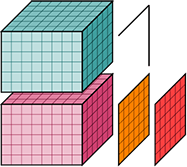
\includegraphics[height=0.15\textwidth]{xarray}
            \end{figure}
            \vspace*{10pt}
        \end{column}
    \end{columns}
\end{frame}

\section{Abstractions}

\begin{frame}{Concepts}
    \vspace*{10pt}
    \begin{center}
        \textbf{Abstractions} are useful because they \textbf{encode concepts}.
    \end{center}
    \vspace*{30pt}

    \begin{columns}
        \begin{column}{0.1\textwidth}
        \end{column}
        \begin{column}{0.4\textwidth}
            \vcinclude{numpy}{height=50pt} {\Huge $\,\quad\to\qquad$} N-dim array
            \vspace*{10pt}

            \vcinclude{pandas}{height=50pt} {\Huge $\qquad\to\qquad$} Table
        \end{column}
        \begin{column}{0.4\textwidth}
            \vcinclude{xarray}{height=50pt} {\Huge $\.\quad\to\qquad$} Dataset
            \vspace*{10pt}

            \vcinclude{networkx}{height=50pt} {\Huge $\qquad\to\qquad$} Network
        \end{column}
        \begin{column}{0.1\textwidth}
        \end{column}
    \end{columns}
    \vspace*{10pt}
    \begin{flushright}
        \footnotesize
        Many useful libraries implement tools to \textbf{perform an action},
        not only to manage data structures.
    \end{flushright}
    \vspace*{10pt}

    It is crucial to \textit{hide} implementation \textit{details}
    ($\sim$ \textbf{encapsulation}).

    Often fundamental for the solution, and understanding them can improve the
    usage.\newline
    But they add a huge cost for the user: hard to learn, depend on the
    internals.

    \begin{flushright}
        \footnotesize
        Check more among NumFOCUS
        \href{https://numfocus.org/sponsored-projects}{sponsored} and
        \href{https://numfocus.org/sponsored-projects/affiliated-projects}{affiliated}
        projects.
    \end{flushright}
\end{frame}

\begin{frame}{Building Blocks}
    \vspace*{20pt}
    \begin{columns}
        \begin{column}{0.5\textwidth}
            On one side Python is a terrible language to build abstractions:
            everything is \textbf{exposed}.
            \begin{figure}
                \centering
                
\includegraphics[width=0.2\textwidth]{capsule}
            \end{figure}

            On the other, it is a perfect one: it relies on \textbf{duck typing}.
            \begin{figure}
                \centering
                
\includegraphics[width=0.3\textwidth]{duck.png}
            \end{figure}

            \begin{center}
                \itshape
                If it looks like a duck, swims like a duck, and quacks like a
                duck, then it is a duck.
            \end{center}
        \end{column}
        \begin{column}{0.5\textwidth}
            Each well-behaving object can be used as an \textbf{effective
            building block} inside a more complex infrastructure.
            \vspace*{20pt}

            \begin{figure}
                \centering
                
\includegraphics[width=0.8\textwidth]{infrastructure}
            \end{figure}
            \vspace*{20pt}

            The essential concept to tame complexity is modularity\footnote{
                Objects are definitely useful, but not mandatory.
            }.
        \end{column}
    \end{columns}
\end{frame}

\section{Interfaces}

\begin{frame}[fragile]{What is an interface?}
    \vspace*{30pt}
    \begin{columns}
        \begin{column}{0.02\textwidth}
        \end{column}
        \begin{column}{0.47\textwidth}
            Some programming languages define an explicit concept of interface:

            \begin{lstlisting}[language=Go,style=mystyle]
// Go example, see full at: https://gobyexample.com/interfaces
type geometry interface {
    area() float64
    perim() float64
}

type rect struct {
    width, height float64
}
// Implement geometry on rects.
func (r rect) area() float64 {
    return r.width * r.height
}
// [...]

// Call methods that are in the named interface.
func measure(g geometry) {
    fmt.Println(g)
    fmt.Println(g.area())
    fmt.Println(g.perim())
}\end{lstlisting}

            In its most basic instance, it is just an object that expose a
            property (also a specific attribute in Plain Old Data, POD).
        \end{column}
        \begin{column}{0.47\textwidth}
            This is intrinsic in OOP, e.g.\ C++\footnote{
                where no explicit interface feature is present
            } gets extremely close through pointers and
            \href{https://en.wikipedia.org/wiki/Polymorphism_(computer_science)}{polymorphism}.

            \begin{lstlisting}[language=C++,style=mystyle]
// C++ example, see full at: https://cplusplus.com/doc/tutorial/polymorphism/
class Polygon {
  protected:
    int width, height;
  public:
    void set_values (int a, int b)
      { width=a; height=b; }
};

class Rectangle: public Polygon {
  public:
    int area()
      { return width*height; }
};

int main () {
  Rectangle rect;
  Polygon * ppoly1 = &rect;
  ppoly1->set_values (4,5);
  cout << rect.area() << '\n';
  return 0;
}\end{lstlisting}
        \end{column}
        \begin{column}{0.02\textwidth}
        \end{column}
    \end{columns}
\end{frame}

\begin{frame}[fragile]{More Abstract}
    \vspace*{30pt}
    \begin{columns}
        \begin{column}{0.5\textwidth}
            Interfaces exists also \textbf{independently from} any specific
            \textbf{language} feature.

            \begin{center}
                \itshape
                They are \alert{contracts} between two or multiple parties, on
                a certain behavior.
            \end{center}

            Consider that the word \enquote{interface} is also in \textit{API
            (application programming interface)} and \textit{ABI (application
            binary interface)}.\newline

            \begin{figure}
                \centering
                
\includegraphics[width=0.5\textwidth]{contract}
            \end{figure}

            E.g. an API is a contract between developers/source codes, while an
            ABI is an agreement at the level of the compiled code.
        \end{column}
        \begin{column}{0.5\textwidth}
            Another example of interface is a \textbf{Foreign Function
            Interface (FFI)}, that is a way to call code from a different
            language (\alert{fundamental in Python}, more later).
            \vspace*{10pt}

            \begin{lstlisting}[language=Python,style=mystyle]
import ctypes
libc = ctypes.CDLL('/lib/libc.so.6')  # Under Linux/Unix
t = libc.time(None)  # Equivalent C code: t = time(NULL)
print(t)\end{lstlisting}
            \vspace*{20pt}

            Interfaces are a concept (or a
            \href{https://refactoring.guru/design-patterns}{design pattern})
            you can also use to build other concepts upon.\newline

            E.g.\ a \href{https://en.wikipedia.org/wiki/Mixin}{mixin}, leverage
            a specific behavior (an interface), to provide some other features
            to your object\footnote{
                Specifically related to OOP and inheritance.
            }.
        \end{column}
    \end{columns}
\end{frame}

\begin{frame}[fragile]{More Interfaces}
    \vspace*{20pt}
    \begin{columns}
        \begin{column}{0.5\textwidth}
            Another option to interface two different programs is to have them
            talking through files.\newline

            An agreement over a \textbf{file structure} is an interface.
            \begin{flushright}
                \footnotesize
                File structure is more than just the language (e.g.\ a
                \texttt{YAML} file).

                \hspace*{10em} The language specify just the
                \textbf{\textit{syntax}}, while a proper interface should
                specify also the \textbf{\textit{semantics}}.
            \end{flushright}

            \begin{figure}
                \centering
                
\includegraphics[width=0.2\textwidth]{data-file}
            \end{figure}

            In general, you can implement the concept \alert{\textbf{in data}},
            e.g.\ including memory exchange of \textit{text} or \textit{binary
            blobs} (think about in memory databases).

            \begin{flushright}
                \footnotesize
                In practice, apart from specific needs, it is convenient to use
                files.
            \end{flushright}
        \end{column}
        \begin{column}{0.5\textwidth}
            An interface can be enforced over a generic data structure, by
            creating suitable methods that \textbf{encapsulate} the underlying
            data.

\begin{lstlisting}[language=Python,style=mystyle]
# not Pythonic, don't use this
class Polygon:
    def __init__(self, kind):
        self.__kind = kind

    def get_kind(self):
        return self.__kind
 
    def set_kind(self, kind):
        self.__kind = kind\end{lstlisting}

            However, methods are useful, but not \textbf{required}.
            When not needed, nor specifically useful, avoid - an instance of
            the
            \href{https://en.wikipedia.org/wiki/Rule_of_least_power}{\enquote{rule
            of least power}}.\newline

            Another option is to make clever use of \textbf{plain functions}
            that act on specific objects.
            \begin{flushright}
                \footnotesize
                \hspace*{15em}Also consider that Python does not allow to split
                methods in many \enquote{blocks} (\texttt{impl} blocks).

                \hspace*{15em}Thus, it is essential to use external functions to
                keep your code \textbf{modular} (divide in files by task).
            \end{flushright}
        \end{column}
    \end{columns}
\end{frame}

\begin{frame}[fragile]{In Python}
    \vspace*{30pt}
    \begin{columns}
        \begin{column}{0.5\textwidth}
            While \textbf{Plain Old Data} are the least powerful object, they
            are \textbf{not available} in Python (since everything is an
            object).
            
            So the best way is to \alert{\textit{limit yourself}}, and do not
            do everything is allowed, e.g.\
            \begin{description}
                \item[attributes] use attributes, not methods
                \item[types] add types to \texttt{\_\_init\_\_()}
                \item[dataclasses] use standard library
                  \href{https://docs.python.org/3/library/dataclasses.html}{\texttt{dataclasses}}
                  module, for better consistency\footnote{
                      Eventually, this will provide you more tools, but also
                      because it enforces a certain layout, so it has more
                      guarantees.
                  }
            \end{description}
            \vspace*{10pt}

            In general, the \textbf{static analyzer} is your best friend
            (analogue to a \textit{compiler}).

            \textbf{Type hints} have \textit{no effect at runtime}, but they
            help a lot in developing and debugging.
            But do not break duck typing!\footnote{
                Unless strictly needed.
                However,
                \href{https://docs.python.org/3/library/typing.html}{\texttt{typing}}
                module provides all the resources for it $\to$ modern
                \textbf{\textit{dynamic typed languages with type hints}} are
                \alert{\textbf{not}} extremely \alert{\textbf{different}} from
                modern \textbf{\textit{statically typed with generics}}, there
                is a convergence.
            }\newline

            Writing \textbf{explicit code} helps the analyses.
        \end{column}
        \begin{column}{0.5\textwidth}
            \href{https://en.wikipedia.org/wiki/Encapsulation_(computer_programming)}{\textbf{Encapsulation}}
            in Python is better done with
            \href{https://docs.python.org/3/library/functions.html#property}{properties}:
            \begin{lstlisting}[language=Python,style=mystyle]
class Polygon:
    def __init__(self, kind):
        self.__kind = kind

    @property
    def kind(self):
        return self.__kind

    @kind.setter
    def kind(self, kind):
        self.__kind = kind\end{lstlisting}
            \vspace*{20pt}


            Also, in Python itself you can find the concept of interface
            (protocol, e.g.\ a
            \href{https://docs.python.org/3/glossary.html\#term-sequence}{sequence})
            implemented at many levels:

            \begin{description}
                \item[C API] at the level of C implementation\footnote{
                        \texttt{CPython} specific
                    }, the
                    \href{https://docs.python.org/3/c-api/sequence.html}{Sequence
                    Protocol}
                \item[typing] in the type hinting system,
                    \href{https://docs.python.org/3/library/typing.html?highlight=sequence\#typing.Sequence}{\texttt{typing.Sequence}}
                \item[runtime] consumable in code itself,
                    \href{https://docs.python.org/3/library/collections.abc.html?highlight=sequence\#collections.abc.Sequence}{\texttt{collections.abc.Sequence}} 

            \end{description}
        \end{column}
    \end{columns}
\end{frame}

\begin{frame}[fragile]{Public Interface}
    \vspace*{30pt}
    \begin{columns}
        \begin{column}{0.03\textwidth}
        \end{column}
        \begin{column}{0.47\textwidth}
            The API is a central concept for a library.

            In particular, each library should define a \alert{\textbf{public
            API}}, and keep it as \textbf{stable as possible}.
            \vspace*{20pt}

            In Python there is \textit{no absolute way to hide}\footnote{
                Guido van Rossum:
                \href{https://therealadam.com/2016/09/26/were-all-adults-here-but-were-not-all-mind-readers/}{\enquote{We're all adults here}}
            } package and
            modules content, but there are a few ways to split public and
            internal elements:

            \begin{description}
                \item[private] modules and packages, i.e.\ scope all internal
                  details under something like \texttt{\_internal}
                \item[export] top-level all the public elements
                \item[\href{https://docs.python.org/3/tutorial/modules.html\#importing-from-a-package}{\texttt{\_\_all\_\_}}]
                    but this pairs with \texttt{from mymod import *}, so I
                    recommend to avoid top level (user facing)
            \end{description}
            \vspace*{20pt}
        \end{column}
        \begin{column}{0.03\textwidth}
        \end{column}
        \begin{column}{0.47\textwidth}
            E.g.\ Numpy's
            \href{https://github.com/numpy/numpy/blob/86cd584b81385508f7d939fc66393a6a27f02659/numpy/__init__.py#L140-L155}{\texttt{\_\_init\_\_.py}}
            looks like:

            \begin{lstlisting}[language=Python,style=mystyle,firstnumber=140]
from . import core
from .core import *
from . import compat
from . import lib
# NOTE: to be revisited following future namespace cleanup.
# See gh-14454 and gh-15672 for discussion.
from .lib import *


from . import linalg
from . import fft
from . import polynomial
from . import random
from . import ctypeslib
from . import ma
from . import matrixlib as _mat
from .matrixlib import *\end{lstlisting}
        So, they are using mostly the \textbf{export} style, but also using
        \texttt{\_\_all\_\_} internally.
        \begin{flushright}
            \footnotesize
            \hspace*{15em}And, in practice, they also make use of
            \textbf{private} modules and subpackages.
        \end{flushright}
        \end{column}
    \end{columns}
\end{frame}

\section{Python Examples}


\begin{frame}[fragile]{Principles}
    \vspace*{20pt}
    \begin{columns}
        \begin{column}{0.02\textwidth}
        \end{column}
        \begin{column}{0.38\textwidth}
            Let's start with some guidance:
            \begin{lstlisting}[language=Python,style=mystyle]
import this\end{lstlisting}
        \end{column}
        \begin{column}{0.6\textwidth}
            \lstset{moredelim=[is][\bfseries]{[*}{*]}}
            \begin{lstlisting}[style=mystyle]
The Zen of Python, by Tim Peters

Beautiful is better than ugly.
[* -> Explicit is better than implicit.*]
Simple is better than complex.
Complex is better than complicated.
Flat is better than nested.
Sparse is better than dense.
[* -> Readability counts.*]
Special cases aren't special enough to break the rules.
Although practicality beats purity.
Errors should never pass silently.
Unless explicitly silenced.
In the face of ambiguity, refuse the temptation to guess.
There should be one-- and preferably only one --obvious way to do it.
Although that way may not be obvious at first unless you're Dutch.
Now is better than never.
Although never is often better than *right* now.
If the implementation is hard to explain, it's a bad idea.
If the implementation is easy to explain, it may be a good idea.
Namespaces are one honking great idea -- let's do more of those!\end{lstlisting}
        \end{column}
    \end{columns}
\end{frame}

\begin{frame}[fragile]{Anti-Patterns}
    \vspace*{30pt}
    \begin{columns}
        \begin{column}{0.5\textwidth}
            Base your interfaces on \textbf{strings} is \textbf{not a good
            idea}.

            Strings are values, so runtime objects: they are unknown for any
            static analyses.

            \begin{lstlisting}[language=Python,style=mystyle]
def myfunc(a: str):
    if a == "ciao":
        # do something

myfunc("ci" + "ao")\end{lstlisting}
            \vspace*{10pt}

            Even more dictionaries: you need to \textit{\textbf{duplicate the
            value}} all over your code, just to access it.

            \begin{lstlisting}[language=Python,style=mystyle]
def myfunc(d: dict) -> int:
    return d["come"] + d["va"]\end{lstlisting}

            Here you just see better what is happening:

            \begin{enumerate}
                \item how can you be sure that \texttt{come} and \texttt{va}
                    are in \texttt{d}?
                \item how can you tell that they are integers?
            \end{enumerate}
            \vspace*{10pt}

            First simple solution: 
            \begin{center}
                \itshape
                if you are dealing with something that is \textbf{abstractly an
                object}, use a \textbf{language object}.
            \end{center}
        \end{column}
        \begin{column}{0.5\textwidth}
            In practice, this means replace \texttt{dict} with a \texttt{class}
            and its attributes\footnote{
                Notice, that in Python objects' attributes are implemented on
                top of \texttt{dict}, that you can always retrieve with
                \texttt{obj.\_\_dict\_\_}. But this is part of the language,
                and Python is aware of it!
            }:


            \begin{lstlisting}[language=Python,style=mystyle]
class MyClass:
    def __init__(self, come: int, va: int):
        self.come = come
        self.va = va

def myfunc(obj: MyClass) -> int:
    return obj.come + obj.va\end{lstlisting}

            Better :)

            You can still do a lot at runtime to mess up, e.g.:
            \begin{description}
                \item[replace] value, with a \enquote{bad} one
                    \begin{lstlisting}[language=Python,style=mystyle]
obj.come = True\end{lstlisting}
                \item[delete] an attribute
                    \begin{lstlisting}[language=Python,style=mystyle]
del obj.come\end{lstlisting}
            \end{description}

            But these operations \alert{can be detected} by a \textbf{static}
            analyzer!
        \end{column}
    \end{columns}
\end{frame}

\begin{frame}[fragile]{Properties}
    \vspace*{20pt}
    \begin{columns}
        \begin{column}{0.5\textwidth}
            Properties can be used with getters and setters to enforce some
            constraint or extra operation.

            \begin{lstlisting}[language=Python,style=mystyle]
class Polygon:
    def __init__(self, kind):
        self.__kind = kind

    @property
    def kind(self):
        # evil self toggling kind
        oldkind = self.__kind
        self.__kind = (
            "triangle" if oldkind != "triangle" else "square"
        )
        return oldkind

    @kind.setter
    def kind(self, kind):
        # notice again the bad use of strings! see enums after
        if kind not in ["triangle", "square", "pentagon"]:
            # use custom errors! another language feature,
            # improve error handling
            raise UnknownPolygonError(kind)
        self.__kind = kind\end{lstlisting}
        \end{column}
        \begin{column}{0.5\textwidth}
            But they do not have to mirror attributes: so they can provide some
            \enquote{virtual} attributes.

            \begin{lstlisting}[language=Python,style=mystyle]
class MyDate:
    def __init__(self, date: str):
        # convention: two leading _ is private, one is protected
        # only double _ will trigger language feature (mangling)
        # see PEP-8#descriptive-naming-styles
        self._date = date

    @property
    def day(self) -> int:
        return int(self._date.split("/")[0])

    @property
    def month(self) -> int:
        return (self._date.split("/")[1])

    @property
    def year(self) -> int:
        return int(self._date.split("/")[2])

MyDate("06/10/2022")\end{lstlisting}

            \begin{flushright}
                \footnotesize
                Notice that \textbf{here} \textbf{\alert{type hints}} are
                \textbf{\alert{not needed}} for properties: that static analyzer
                will work out on its own that the \textbf{return type} is
                \textbf{always an integer}!
            \end{flushright}
        \end{column}
    \end{columns}
\end{frame}

\begin{frame}[fragile]{Dataclasses}
    \vspace*{20pt}
    \begin{columns}
        \begin{column}{0.03\textwidth}
        \end{column}
        \begin{column}{0.47\textwidth}
            Dictionaries can be replaced by objects, but only partially
            satisfactory: \code{\_\_init\_\_} is still an entire function. 
            \begin{flushright}
                \footnotesize
                Just to declare a few attributes!
            \end{flushright}
            \vspace*{10pt}

            Definitely not the least powerful way to do it, Python standard
            library offers a ready-made solution:
            \href{https://docs.python.org/3/library/dataclasses.html}{\code{dataclasses}}
            module.

            \begin{lstlisting}[language=Python,style=mystyle]
import dataclasses

@dataclasses.dataclass
class MyClass:
    ciao: int
    come: str
    va: str = "bene"\end{lstlisting}

            So, we are using the type hints, and a restricted
            \code{\_\_init\_\_} function, to re-engineer missing POD.
        \end{column}
        \begin{column}{0.47\textwidth}
            Another interesting problem is serialization: it is very simple to
            serialize from and deserialize to a \code{dict}.

            \begin{lstlisting}[language=Prolog,style=mystyle]
ciao: 3
come: bene
va: grazie\end{lstlisting}
            
            But what about the \code{dataclass}?

            Also that one can be converted from and to \code{dict}:
            \begin{lstlisting}[language=Python,style=mystyle]
import yaml

with open("myfile.yaml") as fd:
    cnt = yaml.safe_load(fd)

dc = MyClass(**cnt)
print(dc.asdict())\end{lstlisting}

            So a \code{dict} is the best option when you want to load \textbf{everything}.
            But then, if you want to load and validate a specific object (e.g.\
            a runcard), a \code{dataclass} is ideal.
        \end{column}
        \begin{column}{0.03\textwidth}
        \end{column}
    \end{columns}
\end{frame}

\begin{frame}[fragile]{Custom Values \& Enums}
    \vspace*{10pt}
    \begin{center}
        \itshape
        But what about values?
    \end{center}
    \vspace*{20pt}

    \begin{columns}
        \begin{column}{0.03\textwidth}
        \end{column}
        \begin{column}{0.47\textwidth}
            If the object has to follow a certain rule, the best option is to
            go programmatically:

            \begin{lstlisting}[language=Python,style=mystyle]
def condition(val):
    return # my condition

class ConditionType:
    def __init__(self, val):
        if not condition(val):
            raise ConditionError
        self.val = val\end{lstlisting}

            Another option would not be flexible enough, or more involved.

            In this case we need the power, so we use it.
        \end{column}
        \begin{column}{0.47\textwidth}
            But a very common case is a set of finite values:
            \begin{lstlisting}[language=Python,style=mystyle]
from enum import Enum, auto

class FiniteType(Enum):
    VAL1 = auto()
    VAL2 = auto()
    VAL3 = auto()\end{lstlisting}

            The standard library module \code{enum} provides a custom
            metaclass, and other utilities to manage enum types:
            \begin{lstlisting}[language=Python,style=mystyle]
# Test if value is part of type
val in FiniteType
# Values are unique, compare by identity
val is FiniteType.VAL1
# iterate values
list(FiniteType)\end{lstlisting}
        \end{column}
        \begin{column}{0.03\textwidth}
        \end{column}
    \end{columns}
\end{frame}

\begin{frame}[fragile]{Foreign Function Interface}
    \vspace*{30pt}
    \begin{columns}
        \begin{column}{0.5\textwidth}
            \begin{center}
                \itshape
                A foreign function interface (FFI) is a mechanism by which a
                \textbf{program} written \textbf{in one} programming
                \textbf{language} can \alert{\textbf{call routines}} or make
                use of services written \textbf{in another}.
            \end{center}

            I.e.\ it is a way to \textbf{consume a library} from a language in
            a program \textbf{in a different language}.

            This is the basic, but in a sense is not complete: usually provides
            extended or complete bindings for the object in the two languages:
            \begin{itemize}
                \item functions
                \item types
                \item classes
            \end{itemize}
			\vspace*{10pt}

            Python standard library provides
            \href{https://docs.python.org/3/library/ctypes.html}{\code{ctypes}}
            module for FFI with C:
            \begin{lstlisting}[language=Python,style=mystyle]
import ctypes
libc = ctypes.CDLL('/lib/libc.so.6')
t = libc.time(None)
c_s = c_wchar_p("Hello, World")
print(c_s)  # c_wchar_p(139966785747344)
print(c_s.value)  # Hello World
c_s.value = "Hi, there"
print(c_s.value)  # Hi, there
libc.printf(b"Hello, %s\n", b"World!")  # Hello, World!\end{lstlisting}

        \end{column}
        \begin{column}{0.5\textwidth}
            This is possible because Python is
            \href{https://docs.python.org/3/extending/extending.html}{C
            interoperable} (both statically\footnote{
                You can link modules in the interpreter binary, usually for
                standard library.
            } and dynamically\footnote{
                You can load specific dynamic libraries, i.e.\ \code{.so},
                \code{.dylib}, or \code{.dll} files.
            }).

            This is extremely useful, especially for \textbf{performance
            intensive} and \textbf{memory critical} tasks.
            Or for consuming a useful library without reimplementing for
            Python (e.g.\ \href{https://libgit2.org/}{\code{libgit2}}).
            \vspace*{20pt}

            Through C, you can also bind to other languages.
            Here, a brief review of some useful options:

            \begin{description}
                \item[C/C++] \href{https://cython.org/}{Cython} favorite
                    option,
                    \href{https://cffi.readthedocs.io/en/latest/overview.html}{\code{cffi}}
                    alternative
                \item[Rust] \href{https://pyo3.rs/}{PyO3} and
                  \href{https://maturin.rs}{maturin}
                \item[Fortran]
                    \href{https://numpy.org/doc/stable/f2py/}{\code{f2py}},
                    part of \code{numpy}
                \item[\href{https://www.swig.org/}{Swig}] automatic\footnote{
                    It has a
                    \href{https://www.swig.org/compat.html\#SupportedLanguages}{broader
                    scope} than Python.
                  }, but mostly
                  painful because of manual patching often required
            \end{description}
            \vspace*{20pt}
        \end{column}
    \end{columns}
\end{frame}

\begin{frame}[fragile]{Rust Example}
    \vspace*{20pt}
    \begin{columns}
        \begin{column}{0.5\textwidth}
            Project structure:
            \begin{lstlisting}[style=mystyle]
Cargo.lock
Cargo.toml
mypypkg/
    __init__.py
pyproject.toml
src/
    lib.rs\end{lstlisting}
            \vspace*{10pt}

            Python layer available: you can customize from the Python side, it
            can be easier and results in more Pythonic interface.
            \begin{lstlisting}[language=Python,style=mystyle]
# __init__.py
from . import mypypkg

class MyAdder:
    def __init__(self, l: list[float]):
        self.buffer = l

    def add(self) -> float:
        return mypypkg.add(self.buffer)\end{lstlisting}
        \end{column}
        \begin{column}{0.5\textwidth}
            And here instead the Rust side implementation: you can also use
            whatever other Rust crate (library) in here.
            \begin{lstlisting}[language=C++,style=mystyle]
// lib.rs
use pyo3::prelude::*;

/// Add a sequence of floats.
#[pyfunction]
fn add(v: Vec<f64>) -> PyResult<f64> {
    Ok(v.iter().sum())
}

/// A Python module implemented in Rust.
#[pymodule]
fn mypypkg(_py: Python, m: &PyModule) -> PyResult<()> {
    m.add_function(wrap_pyfunction!(add, m)?)?;
    m.add("version", env!("CARGO_PKG_VERSION"))?;

    Ok(())
}\end{lstlisting}

            For more info (and more clever examples) see
            \href{https://pyo3.rs/v0.17.1/getting_started.html#running-code}{PyO3}
            and
            \href{https://maturin.rs/project_layout.html#mixed-rustpython-project}{maturin
            guide}.
        \end{column}
    \end{columns}
\end{frame}

\section{Project Management}

\begin{frame}{Docs}
    \vspace*{20pt}
    \begin{center}
        Presenting the code is fundamental: since you \textbf{want to have
        users}, it has to be \textit{useful} and \textit{simple}.

        \textit{And everything is \textbf{simple, when} it is
        \alert{\textbf{well explained}}.}
    \end{center}
    \vspace*{10pt}

    \begin{columns}
        \begin{column}{0.35\textwidth}
            It is a synthetic replacement for office hours.
            \vspace*{10pt}

            \begin{itemize}
                \item given a \textbf{question}, the \textbf{answer} should be
                  properly written in the docs; in familiar terms, and simple
                  to find, not only: 
                \item sometimes, it should provide \textbf{answers before
                  questions} (since it is not always clear which are the proper
                  ones)
            \end{itemize}

            \begin{figure}
                \centering
                
\includegraphics[width=0.6\textwidth]{question-docs}
            \end{figure}
        \end{column}
        \begin{column}{0.35\textwidth}
            Good documentation have to provide resources for different users,
            so they need to be \textbf{hierarchical}.
            \vspace*{10pt}

            \begin{description}
                \item[presentation] a \textbf{home page}, to meet new users,
                    and a starting point
                \item[getting started] \textbf{tutorials}, to begin hands on
                \item[user manual] to answer most of the common needs
                \item[reference] a complete explanation of the public interface
            \end{description}
        \end{column}

        \begin{column}{0.3\textwidth}
            \begin{figure}
                \centering
                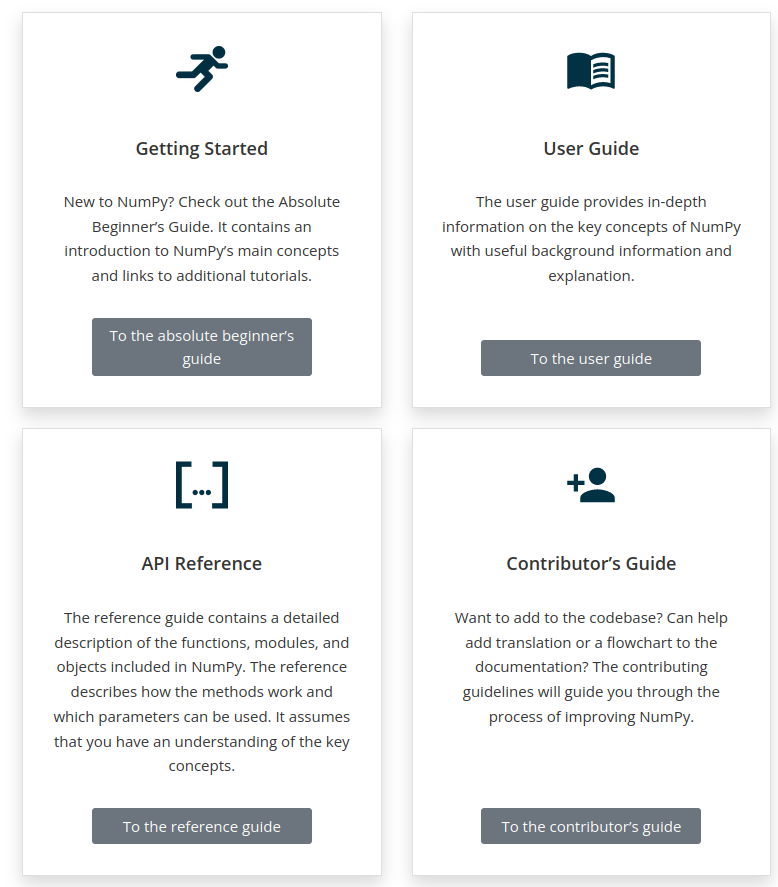
\includegraphics[width=\textwidth]{numpy-hierarchical-docs}
                \caption{
                    Numpy docs \href{https://numpy.org/doc/stable/}{starting page}.
                }
            \end{figure}

            % In general, it is convenient to document everything (e.g.\ with
            % docstrings), but the internals are for developers and
            % maintainability, not for users\footnote{
                % There should be a clear distinction, but they are both
                % important.
            % }.
            % \vspace*{10pt}
        \end{column}
    \end{columns}
\end{frame}

\begin{frame}{Home and Tutorials}
    \begin{columns}
        \begin{column}{0.5\textwidth}
            \vspace*{5pt}

            A good landing page is fundamental:
            \begin{itemize}
                \item a \textbf{unique reference} point
                \item communicate the \textbf{target audience}, and
                \item the scope and \textbf{goal} of the project
            \end{itemize}

            \begin{figure}
                \centering
                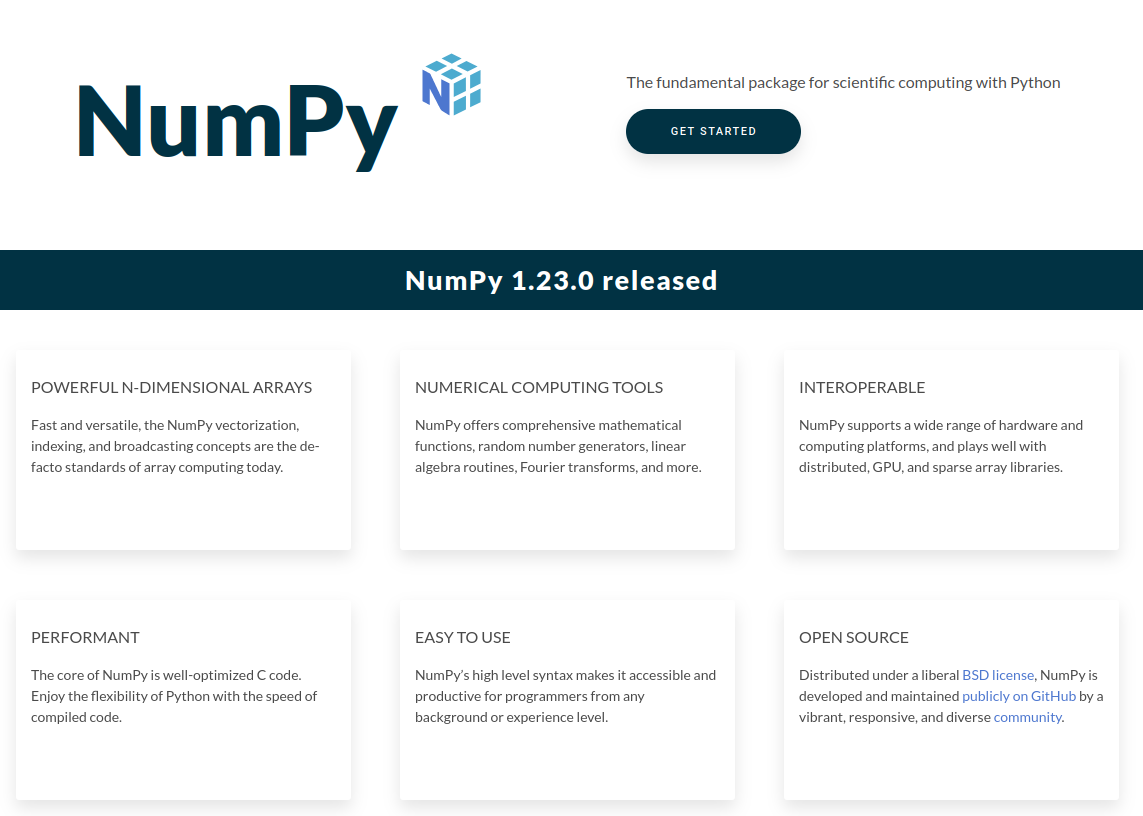
\includegraphics[width=0.8\textwidth]{numpy-home}
                \caption{Numpy \href{https://numpy.org/}{home}.}
            \end{figure}
            
            All the \textbf{relevant pointers} should be here, but only top
            level (think of a \textit{logarithmic navigation}).
        \end{column}
        \begin{column}{0.5\textwidth}
            \vspace*{10pt}

            \textbf{Tutorials} should be a \textit{\textbf{walk-through}}, the
            user has to know nothing but the initial problem.
            \vspace*{5pt}

            Jupyter notebooks are very useful, with explanations and outputs.
            \vspace*{5pt}

            \begin{figure}
                \centering
                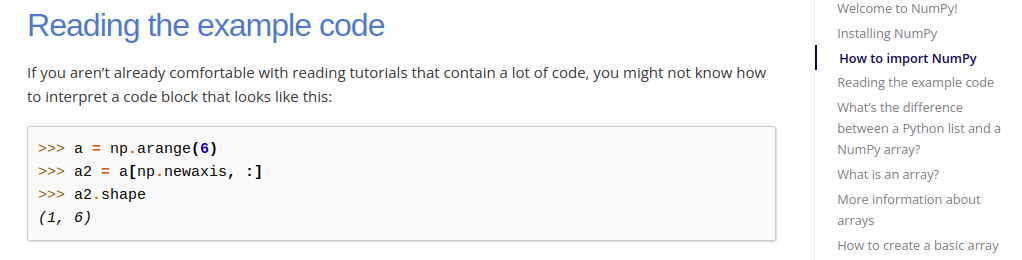
\includegraphics[width=0.9\textwidth]{numpy-abs-beginners}
                \caption{
                    Numpy
                    \href{https://numpy.org/doc/stable/user/absolute_beginners.html}{absolute
                    beginners} guide.
                }
            \end{figure}

            Consider to incrementally collect good examples. If easily
            discoverable they can be extremely useful.
            \vspace*{5pt}

            \begin{figure}
                \centering
                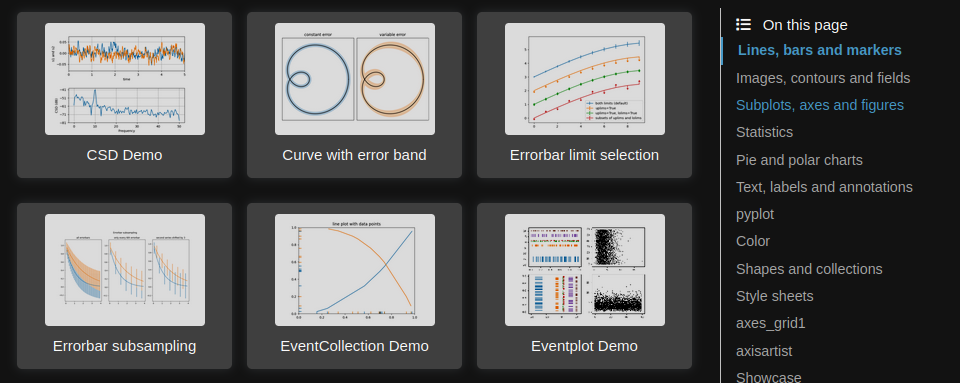
\includegraphics[width=0.8\textwidth]{matplotlib-gallery}
                \caption{
                    Matplotlib
                    \href{https://matplotlib.org/stable/gallery/}{gallery}
                }
            \end{figure}
        \end{column}
    \end{columns}
\end{frame}

\begin{frame}{Dependencies}
    \vspace*{20pt}
    \begin{columns}
        \begin{column}{0.5\textwidth}
            Another crucial point is \textbf{dependencies picking}.
            \vspace*{10pt}

            Trade-off:
            \begin{description}
                \item[pro] software reuse: deduplication, leverage other people work
                \item[con] sync versions, rely on external maintenance
            \end{description}
            \vspace*{20pt}

            So, what if one wants the \textbf{\textsc{pros}} and not the
            \textbf{\textsc{cons}}?

            Mitigate the issues with \textit{optimal choices}:
            \begin{itemize}
                \item \alert{\textbf{community}} or company projects (not
                  single maintainer)
                \item \alert{\textbf{stable}} enough (not early stage)
                \item still \alert{\textbf{active}} (not abandoned)
            \end{itemize}
            \vspace*{10pt}

            The other option is to pick a project, though unstable or inactive,
            and accept to maintain it yourself, in case you need.
        \end{column}
        \begin{column}{0.5\textwidth}
            \begin{figure}
                \centering
                \begin{tcolorbox}[size=tight,sharpish corners,boxrule=0mm]
                    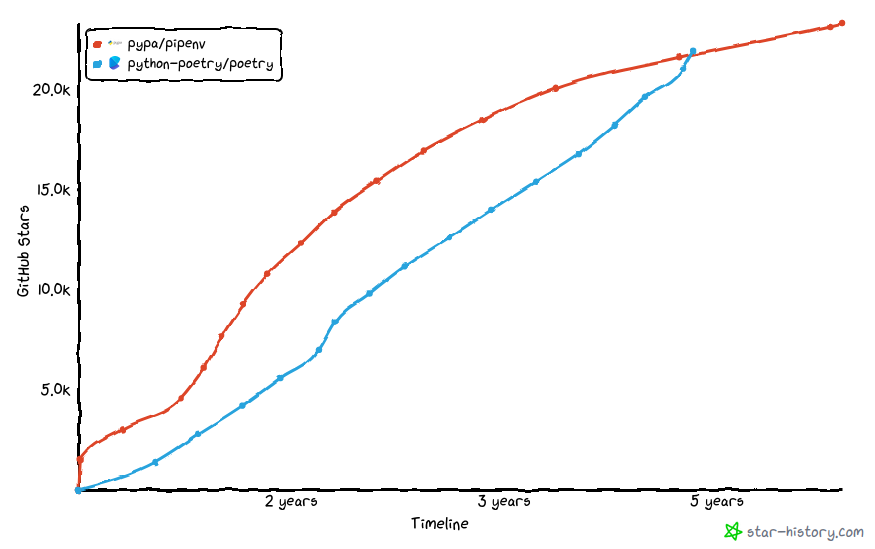
\includegraphics[width=\textwidth]{poetry-vs-pipenv}
                \end{tcolorbox}
                \caption{
                    Both a dependency managers comparison, and a good example
                    of trade-off: Pipenv is older, but Poetry has traction.
                }
            \end{figure}
        \end{column}
    \end{columns}
\end{frame}

\begin{frame}{Bots \& Hooks}
    \vspace*{20pt}
    \begin{columns}
        \begin{column}{0.05\textwidth}
        \end{column}
        \begin{column}{0.45\textwidth}
            Bots are useful as a category: checks that run automatically (and
            often asynchronously, events triggered) on the server.
            \vspace*{15pt}

            A useful example: scan dependencies and get updates about reported
            vulnerabilities.
            \vspace*{5pt}

            \vcinclude{dependabot}{width=50pt}
            \href{https://github.com/dependabot}{\textbf{Dependabot}}:
            Automated
            dependency updates.

            \href{https://probot.github.io/}{\textbf{Probot}}: an entire kit to
            build GitHub apps.
            \vcinclude{probot}{width=50pt}
            \vspace*{5pt}

            {\itshape\small
                I never used myself, but if you need something like Dependabot,
                you can use it to make your custom one (workflows can already
                do a lot).
            }
        \end{column}
        \begin{column}{0.45\textwidth}
            \begin{figure}
                \centering
                
\includegraphics[width=0.4\textwidth]{hooks}
            \end{figure}
            \href{https://git-scm.com/book/en/v2/Customizing-Git-Git-Hooks}{Git
            hooks} are another important help to \textbf{automate} and
            \textbf{ensure} routine \textbf{maintenance} (formatting, checks,
            \dots).\newline

            They are simple \textbf{executable scripts}\footnote{
                Not automatically installed at clone time, not to run unknown
                code.
            }, triggered by Git events (built-in feature, active as client and
            server).
            \vspace*{10pt}

            \href{https://pre-commit.com/}{\texttt{pre-commit}} is a framework
            to manage them.
            \vcinclude{pre-commit}{width=50pt}
            \vspace*{10pt}

            It is absolutely not required, but makes it much simpler to reuse
            hooks (especially community popular ones).
            Almost a \enquote{package manager for pre-commit hooks}.
            \vspace*{15pt}
        \end{column}
        \begin{column}{0.05\textwidth}
        \end{column}
    \end{columns}
\end{frame}

\begin{frame}[standout]
    Thanks for your attention!
\end{frame}

\appendix

\begin{frame}[fragile]{Poetry tutorial \& references}
    \begin{columns}
        \begin{column}{0.03\textwidth}
        \end{column}
        \begin{column}{0.47\textwidth}
            There are many ways to install Poetry, but at this point the most
            convenient is the
            \href{https://python-poetry.org/docs/#installation}{official
            installer}.\newline

            You can find this and other basic information on the website
            \href{https://python-poetry.org/}{home page}.\newline

            Now, there is also an official
            \href{https://python-poetry.org/docs/plugins/}{plugin system}, look
            for them on GitHub, with the tag
            \href{https://github.com/topics/poetry-plugin}{\code{poetry-plugin}}.
        \end{column}
        \begin{column}{0.1\textwidth}
        \end{column}
        \begin{column}{0.4\textwidth}
            \begin{lstlisting}[language=bash,style=mystyle]
# install dependencies
poetry install
# add dependency
poetry add mypackage
# add dependency to given group
poetry add mypackage -G mygroup

# generate lockfile
poetry lock
# update dependencies
poetry update

# run command in environment
poetry run mycommand
# enter shell inside environment
poetry shell\end{lstlisting}
        \end{column}
    \end{columns}
\end{frame}


\begin{frame}{Store Knowledge}
    \vspace*{20pt}
    \begin{columns}
        \begin{column}{0.5\textwidth}
            Storing documents and notes in a project container is definitely
            useful. Wikis are a quite popular solution.\newline

            But when a bunch of people are working together, you start having
            the need to manage it. At that point than having internal wiki $\to$
            internal Q\&A.

            Use \href{https://docs.github.com/en/discussions}{GitHub
            discussions} for this.
            \vspace*{10pt}

            \begin{figure}
                \centering
                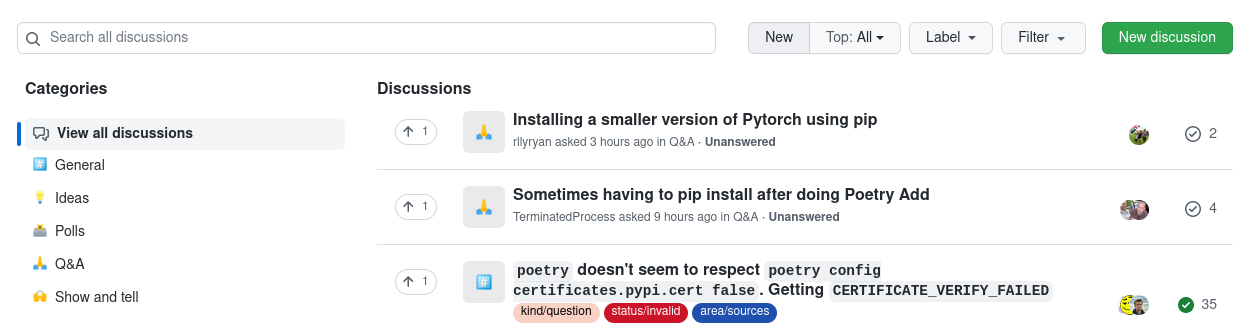
\includegraphics[width=\textwidth]{discussions}
            \end{figure}
            \vspace*{10pt}

            When a colleague give you an answer: consider to write it down in
            the discussions (for your future self, and the other colleagues).

            Sometimes might be handy also to just ask the question directly in
            a discussion.
        \end{column}
        \begin{column}{0.5\textwidth}
            When things consolidate:

            \begin{description}
                \item[\emoji{star} favorite] add to the docs (even developers docs)
                \item[internal] to keep internal add to a
                    \href{https://docs.github.com/en/communities/documenting-your-project-with-wikis/about-wikis}{wiki
                    repository} (also on GitHub)
                \begin{itemize}
                    \item but better to put stuffs properly in an actual
                        repository
                \end{itemize}
            \end{description}

            In case: also
            \href{https://docs.github.com/en/issues/planning-and-tracking-with-projects/learning-about-projects/about-projects}{Projects}
            might be useful, to have a board for discussing status and
            priorities.
            \vspace*{10pt}

            \begin{figure}
                \centering
                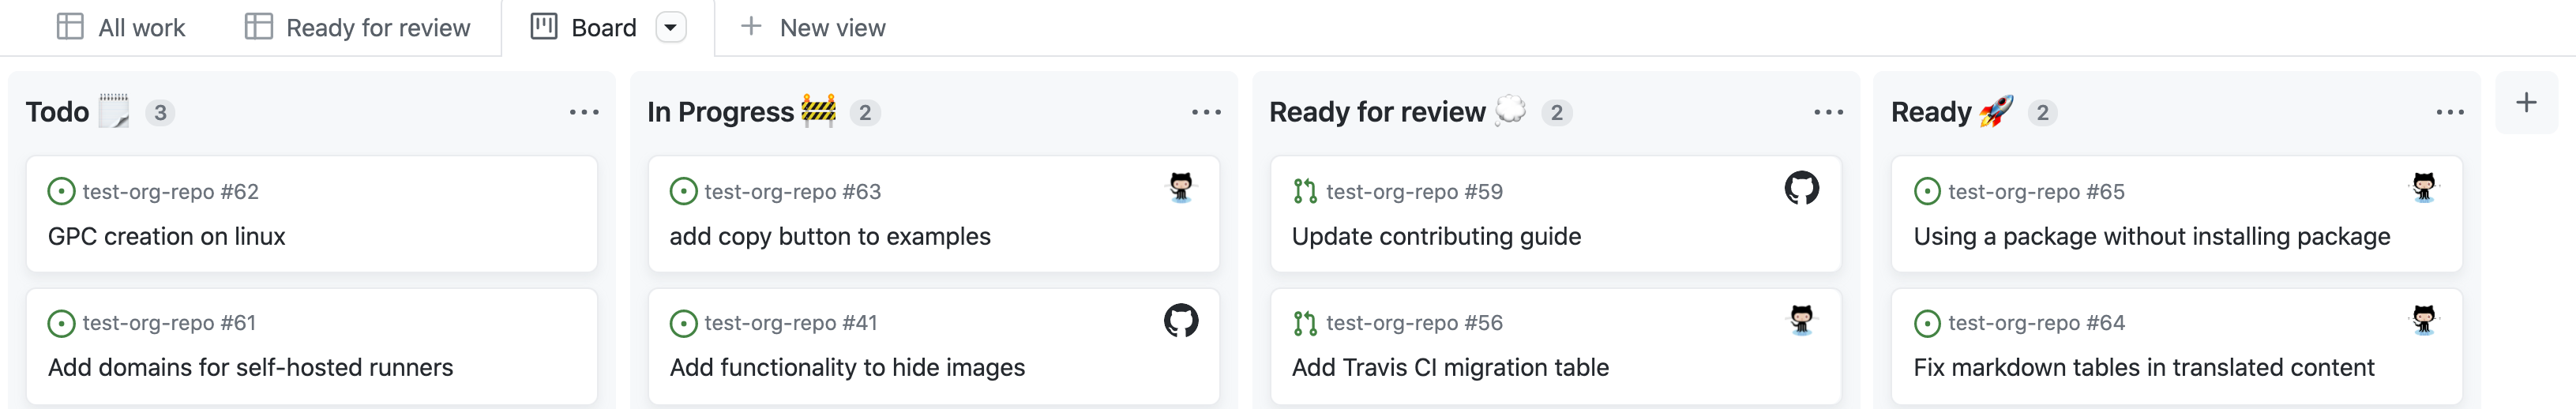
\includegraphics[width=\textwidth]{board}
                \vspace*{10pt}
                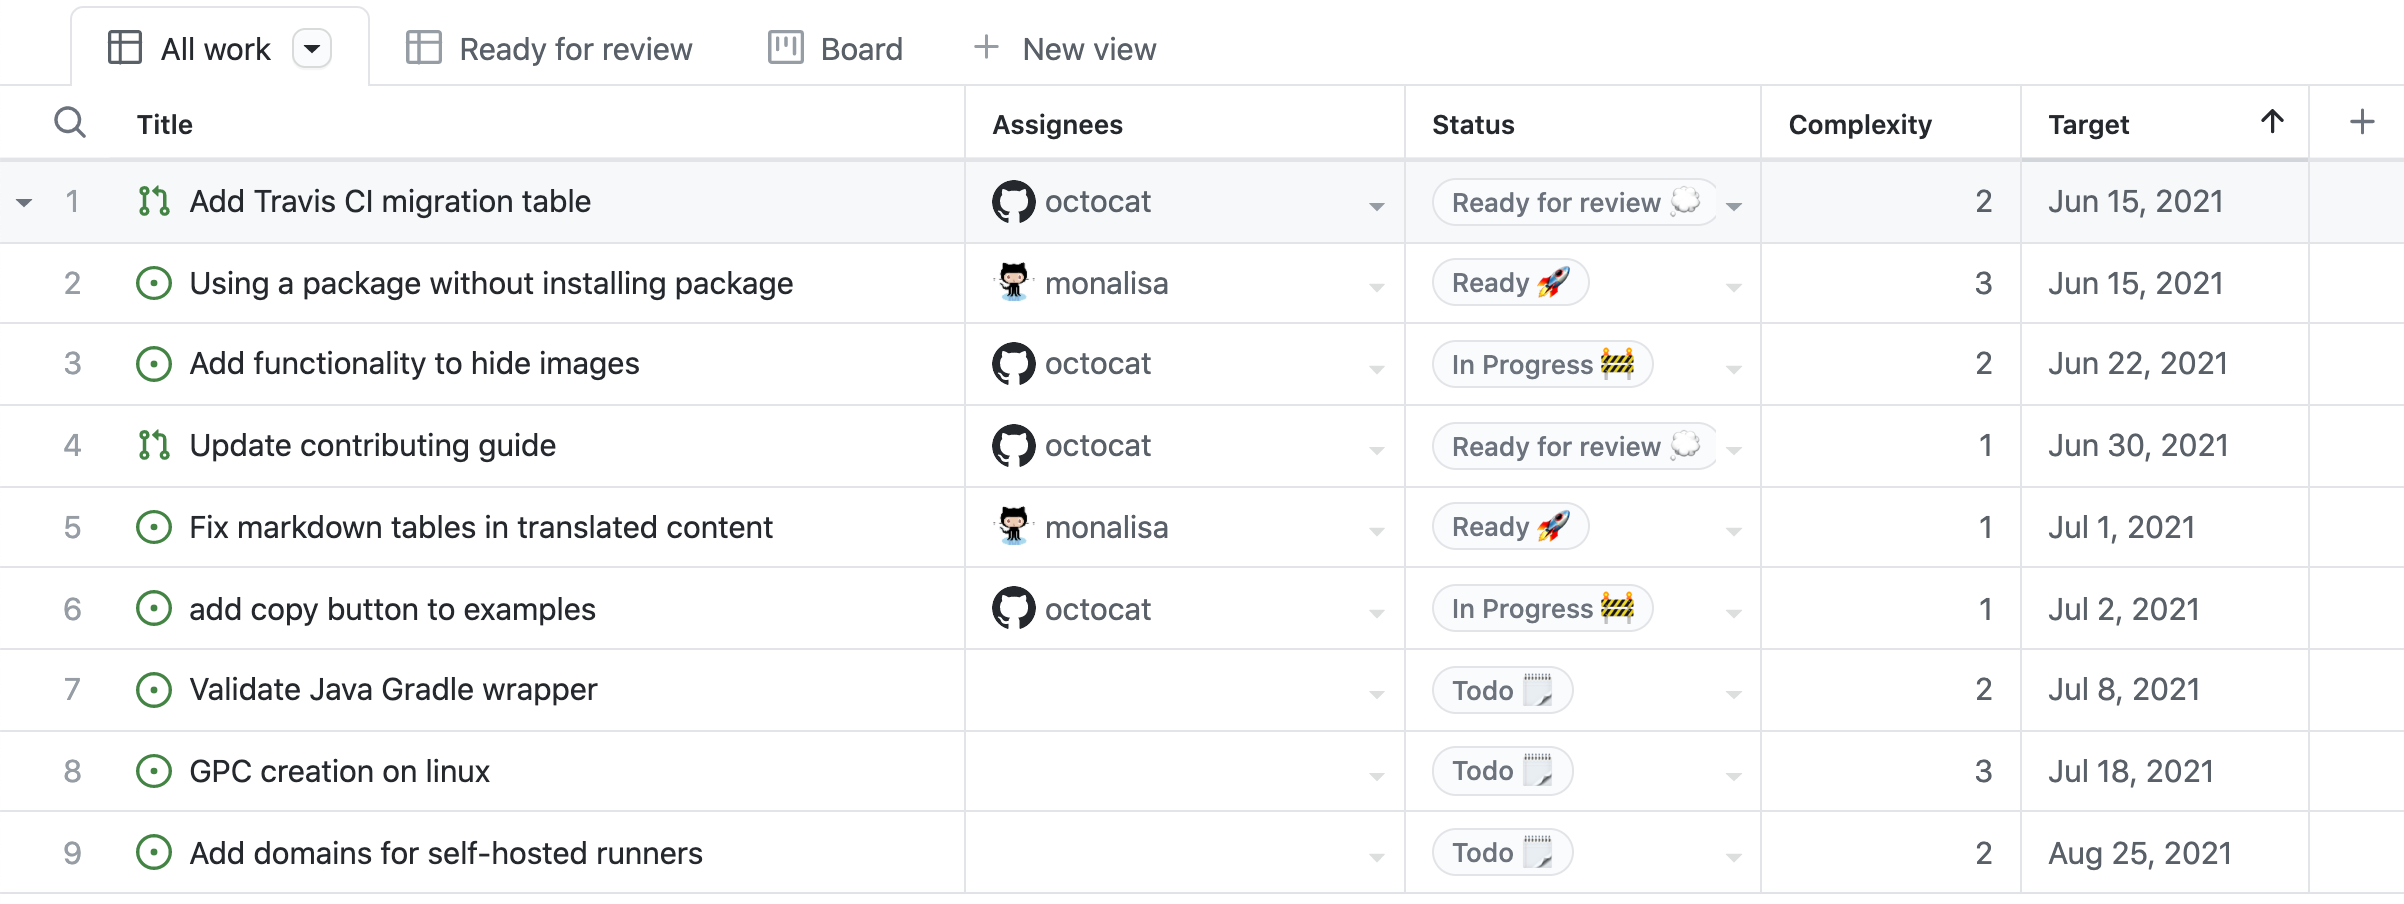
\includegraphics[width=0.7\textwidth]{spreadsheet}
            \end{figure}
        \end{column}
    \end{columns}
    \vspace*{10pt}

    \begin{center}
    And in this way, you have the advantage of having everything in a single
    place.\\
    Otherwise you fragment and start loosing pieces (or their effectiveness).
    \end{center}
\end{frame}


\end{document}
